\begin{nice-box}[Vorlesungsübersicht \& Kontext]
In dieser elften Vorlesungswoche der Graphentheorie vertiefen wir zentrale Konzepte der Graphenstrukturen und deren Anwendungen:
\begin{itemize}
    \item \textbf{Das Handschlaglemma:} Formaler Beweis und alltägliche Interpretation.
    \item \textbf{Euler-Linien \& Euler-Graphen:} Charakterisierung durch den Satz von Euler und Anwendung auf das Dominoproblem.
    \item \textbf{Hamilton-Kreise:} Definition, platonische Körper und die Existenz von Gray-Codes im $k$-dimensionalen Hyperwürfel.
    \item \textbf{Bipartite Graphen \& Heiratssatz von Hall:} Nachbarschaftsmengen und der Heiratssatz als fundamentales Resultat der diskreten Mathematik.
\end{itemize}
\end{nice-box}

\section{Das Handschlaglemma}

\begin{spoken-clean}[00:00:00 - 00:01:58]
Hallo zusammen, wir fangen an. Herzlich willkommen zur \textbf{11.} Woche. Wir sind noch mittendrin in der Graphentheorie --- also ein ganz kleiner Einblick in ein bisschen, um was es in der Graphentheorie, Teilen der Graphentheorie geht.

Letzte Woche haben wir noch kurz mit dem einen Lemma aufgehört. Ich wollte das noch kurz umformulieren: Dieses Lemma heißt auch das Handschlaglemma. \inlinemetanote{schreibt an die Tafel} Das Schöne an der Graphentheorie ist, man kann sie oft so in alltägliche Situationen umformen --- oder viele Sachen sind vielleicht auch Probleme aus dem realen Leben ---, und dann kann man, wenn man sieht, dass das einfach ein Graphenproblem ist, das mit irgendeinem graphentheoretischen Lemma lösen.

Das Handschlaglemma sagt: Auf einer Party mit $n$ Gästen ist die Anzahl der Gäste, die einer ungeraden Anzahl von Gästen die Hand geben, gerade. Okay, und das war im Prinzip genau das, was wir am Ende der letzten Stunde bewiesen haben.

Der Beweis ist: \inlinemetanote{schreibt an die Tafel} Wir betrachten einfach den Graphen $G = (V, E)$, wobei $V$ genau die Gäste sind, und $E$ --- da es ein ungerichteter Graph ist --- einfach die Paare von Gästen sind, die sich die Hand geben. Und wir haben gesehen, dass die Anzahl der $x \in V$, sodass der Grad von $x$ ungerade ist, immer gerade ist.

Vielleicht, okay, wir gehen natürlich davon aus, dass sich die Leute nicht selbst die Hand schütteln. Das geht nicht. Oder wenn man sich selbst die Hand schüttelt, dann zählt das wie zweimal die Hand schütteln, weil man sich ja selbst quasi die Hand geschüttelt hat. Also machen wir nicht. Also einfach nur, um zu sagen, dass das der Fall ist --- gut, sich eine konkrete Situation von gewissen Resultaten vorzustellen.
\end{spoken-clean}

\begin{math-stroke}[Das Handschlaglemma]
\begin{lemma}[Handschlaglemma]\label{lem:handschlaglemma}
Auf einer Party mit $n$ Gästen ist die Anzahl Gäste, die einer ungeraden Anzahl von Gästen die Hand geben, gerade.
\end{lemma}

\begin{short-proof}
Wir modellieren die Situation durch einen ungerichteten Graphen $G = (V, E)$ mit:
\begin{itemize}
    \item \textbf{Knotenmenge $V$:} $V := \{\text{Gäste}\}$,
    \item \textbf{Kantenmenge $E$:} $E := \{\{x, y\} \mid x \text{ und } y \text{ geben sich die Hand}\}$.
\end{itemize}
Da die Summe der Grade aller Knoten in jedem endlichen Graphen stets gerade ist (nämlich gleich $2|E|$), muss die Anzahl der Knoten mit ungeradem Grad ebenfalls gerade sein:
\[
\left| \{ x \in V \mid \deg(x) \text{ ungerade} \} \right| \in 2\mathbb{N}.
\]
Dies beweist die Behauptung.
\end{short-proof}
\end{math-stroke}

\section{Euler-Linien und Euler-Graphen}
\subsection{Definitionen und Charakterisierung}

\begin{spoken-clean}[00:01:58 - 00:04:10]
Und das Letzte, wofür wir letzte Woche leider keine Zeit mehr hatten, war noch diese Sache mit den Euler-Linien. Das ist die folgende Definition: Eine Euler-Linie eines Graphen $G$ ist ein geschlossener Kantenzug, der sämtliche Kanten von $G$ enthält. \inlinemetanote{schreibt an die Tafel}

Okay, also wir hatten Kantenzüge nur für Graphen mit nur einer Relation definiert, aber man kann das ähnlich auch für Graphen mit Mehrfachkanten definieren --- haben wir aber nicht gemacht, das wäre einmal hier. Und es ist wirklich ein Kantenzug, das heißt, jede Kante kommt höchstens einmal vor im Kantenzug. Es dürfen aber dieselben Knoten mehrmals verwendet werden.

Und genau, wenn man einen geschlossenen Kantenzug hat, der alle Kanten von $G$ enthält, dann ist das eine eulersche Linie --- ich schreibe lieber Euler-Linie ---, also ganz gemäß dem Königsberger Brückenproblem. Und ein Graph heißt Euler-Graph, wenn er eine Euler-Linie enthält. \inlinemetanote{schreibt an die Tafel}

Okay. Also der Graph der Königsberger Brücken wäre also ein Beispiel für einen Graphen, der kein Euler-Graph ist, wohingegen das Haus vom Nikolaus ein Graph ist, der ein Euler-Graph ist, wie wir letztes Mal kurz am Anfang als Motivation diskutiert haben. Und das können wir hier noch in dieser Proposition abschließen --- das ist die Proposition \textbf{9.3}.
\end{spoken-clean}

\begin{math-stroke}[Definition der Euler-Linie und des Euler-Graphen]
\begin{definition}[Euler-Linie und Euler-Graph]\label{def:euler-linie}
Sei $G = (V, E)$ ein Graph.
\begin{itemize}
    \item Eine \newterm{Euler-Linie} von $G$ ist ein geschlossener Kantenzug, der sämtliche Kanten von $G$ enthält.
    \item Ein Graph $G$ heißt \newterm{Euler-Graph}, wenn er eine Euler-Linie besitzt.
\end{itemize}
\end{definition}
\end{math-stroke}

\begin{spoken-clean}[00:04:10 - 00:06:20]
Die sagt, dass ein endlicher, ungerichteter, zusammenhängender Graph... zusammenhängend haben wir, glaube ich, nicht definiert. Das heißt einfach das, was man denkt: Wenn man je zwei Knoten nimmt, dann existiert ein Kantenzug zwischen diesen Knoten. Man kann also je zwei Knoten miteinander verbinden --- das ist die Definition, das heißt, es existiert ein Kantenzug zwischen je zwei Knoten. \inlinemetanote{schreibt an die Tafel}

Also ein endlicher, ungerichteter, zusammenhängender Graph $G$ ist genau dann ein Euler-Graph, wenn jeder Knoten von $G$ geraden Grad hat. \inlinemetanote{schreibt an die Tafel}

Das ist der Satz von Euler, mit dem er gezeigt hat, dass eben das Königsberger Brückenproblem keine Lösung hat, weil man dort halt eben viele Knoten hat, die ungeraden Grad haben. Okay? Und die andere Sache ist: Es zeigt nicht nur... okay, Euler hat gesehen, das ist eine notwendige Bedingung, also wenn es ein Euler-Graph ist, dann muss diese Bedingung erfüllt sein. Aber das ist eben auch eine hinreichende Bedingung: Wenn alle Knoten einen geraden Grad haben, dann gibt es eine Euler-Linie.
\end{spoken-clean}

\begin{math-stroke}[Charakterisierung von Euler-Graphen]
\begin{definition}[Zusammenhängender Graph]\label{def:zusammenhaengend}
Ein Graph $G = (V, E)$ heißt \newterm{zusammenhängend}, wenn zwischen je zwei Knoten $x, y \in V$ ein Kantenzug existiert.
\end{definition}

\begin{proposition}[Satz von Euler]\label{prop:satz-von-euler}
Ein endlicher, ungerichteter, zusammenhängender Graph $G$ ist genau dann ein Euler-Graph, wenn jeder Knoten von $G$ geraden Grad hat.
\end{proposition}
\end{math-stroke}

\subsection{Beweis des Satzes von Euler}

\begin{spoken-clean}[00:06:20 - 00:08:30]
Okay. Ja, der Beweis ist im Wesentlichen einfach das Argument von Euler. Falls $G$ eine Euler-Linie hat, so ist jeder Knoten von $G$ von geradem Grad, weil er so oft Anfangs- wie Endpunkt dieser Linie ist. \inlinemetanote{schreibt an die Tafel} Und genau, daraus folgt, dass jeder Knoten einen geraden Grad hat.

Und für die Umkehrung beziehungsweise die Rückrichtung konstruieren wir so eine Euler-Linie, wenn wir wissen, dass das der Fall ist. Zuerst einmal, okay, er ist zusammenhängend; und wenn der Graph zusammenhängend ist, dann heißt das insbesondere, dass es keine Knoten gibt von Ordnung Null (d.\,h.\ isolierte Knoten). Wenn ein Knoten von Ordnung Null wäre, dann könnte man ihn mit niemandem verbinden. Das heißt, jeder Knoten hat mindestens Grad \textbf{2}. \inlinemetanote{schreibt an die Tafel}
\end{spoken-clean}

\begin{math-stroke}[Beweis des Satzes von Euler (Teil 1)]
\begin{short-proof}[Beweis von \cref{prop:satz-von-euler}]
\textbf{Hinrichtung ($\implies$):}
Falls $G$ eine Euler-Linie besitzt, so ist jeder Knoten $v \in V$ von geradem Grad. Da die Euler-Linie ein geschlossener Kantenzug ist, tritt sie bei jedem Durchgang durch einen Knoten $v$ über eine Kante ein und über eine andere Kante wieder aus. Da jede Kante genau einmal durchlaufen wird, ist jeder Knoten $v$ genau so oft Anfangs- wie Endpunkt einer Kante der Linie. Somit ist der Grad jedes Knotens gerade.
\end{short-proof}
\end{math-stroke}

\begin{spoken-clean}[00:08:30 - 00:11:00]
Und was wir jetzt tun: Wir nehmen einen Knoten $x_0$. Wir starten jetzt an einem Knoten $x_0$, wir beginnen jetzt bei $x_0$, und jetzt laufen wir einfach los zu irgendeinem anderen Knoten $x_1$, $x_2$ und so weiter. Und zwar starten wir im Knoten $x_0$, und dann gehen wir vom Knoten $x_i$ weiter zum Knoten $x_{i+1}$ --- und das immer auf einer Kante, die wir noch nicht besucht haben, also auf einer, sagen wir mal, unbesuchten Kante. \inlinemetanote{schreibt an die Tafel}

Und das können wir immer, weil wenn wir auf einer unbesuchten Kante in einen Knoten reingehen, dann gibt es auch noch eine unbesuchte Kante, die wieder rausgeht, weil sonst hätte der entsprechende Knoten ja eine ungerade Ordnung (d.\,h.\ einen ungeraden Grad).

Okay, und jetzt irgendwann kommen wir... also $G$ ist ein endlicher Graphen. Das heißt, wir kommen irgendwann zurück zu $x_0$. \inlinemetanote{schreibt an die Tafel} Das heißt, es existiert ein geschlossener Kantenzug --- $K_0$ nennen wir ihn --- beginnend in $x_0$. Okay, und falls dieser $K_0$ jetzt bereits alle Kanten enthält, ist gut, dann sind wir fertig.
\end{spoken-clean}

\begin{math-stroke}[Beweis des Satzes von Euler (Teil 2)]
\begin{short-proof}[Rückrichtung ($\impliedby$)]
\textbf{Schritt 1: Konstruktion eines ersten geschlossenen Kantenzugs $K_0$}
Da $G$ zusammenhängend ist und jeder Knoten geraden Grad hat, besitzt jeder Knoten mindestens Grad $2$. Wir starten an einem beliebigen Knoten $x_0 \in V$ und konstruieren einen Pfad, indem wir sukzessive über unbesuchte Kanten laufen: 
\[
x_0 \to x_1 \to x_2 \to \dots \to x_i \to x_{i+1}.
\]
Da jeder Knoten geraden Grad hat, besitzt jeder besuchte Zwischenknoten nach dem Betreten stets noch mindestens eine unbesuchte Kante zum Verlassen. Da der Graph $G$ endlich ist, muss dieser Prozess nach endlich vielen Schritten abbrechen, was nur durch die Rückkehr zum Startknoten $x_0$ geschehen kann. Somit erhalten wir einen geschlossenen Kantenzug $K_0$ beginnend in $x_0$.
\end{short-proof}
\end{math-stroke}

\begin{spoken-clean}[00:11:00 - 00:13:30]
Okay, wenn es jetzt aber noch Kanten gibt, die nicht in $K_0$ enthalten sind, dann muss einer der Knoten, die auf $K_0$ liegen, an eine solche Kante angrenzen, weil der Graph ja zusammenhängend ist. Es kann also nicht sein, dass alle unbesuchten Kanten nicht an die Knoten in $K_0$ angrenzen.

Ansonsten gibt es auf $K_0$ einen Knoten $x_1$, von dem natürlich eine gerade Anzahl von Kanten ausgeht, die nicht auf $K_0$ liegen. \inlinemetanote{schreibt an die Tafel und zeichnet ein Diagramm}
\end{spoken-clean}

\begin{math-stroke}[Beweis des Satzes von Euler (Teil 3)]
\begin{short-proof}[Rückrichtung ($\impliedby$) - Fortsetzung]
\textbf{Schritt 2: Erweiterung des Kantenzugs bei unvollständiger Abdeckung}
Falls $K_0$ noch nicht alle Kanten von $G$ enthält, existiert wegen des Zusammenhangs von $G$ mindestens eine unbesuchte Kante, die an einen Knoten $x_1 \in K_0$ angrenzt. Da $K_0$ an jedem Knoten eine gerade Anzahl von Kanten verbraucht, hat $x_1$ bezüglich der verbleibenden unbesuchten Kanten immer noch einen geraden Grad.
\end{short-proof}
\end{math-stroke}

\begin{spoken-clean}[00:13:30 - 00:15:10]
Okay, also wir machen jetzt hier genau dasselbe noch einmal und erhalten hier irgendeinen anderen geschlossenen Kantenzug. Okay, und jetzt können wir einfach die zwei zusammenhängen: Jetzt gehen wir zuerst hier entlang, dann machen wir diesen neuen Kantenzug, und dann machen wir wieder den Rest des ersten Kantenzugs fertig --- dann haben wir einen neuen Kantenzug, der größer ist. \inlinemetanote{schreibt an die Tafel und zeichnet Diagramme}
\end{spoken-clean}

\begin{math-stroke}[Beweis des Satzes von Euler (Teil 4)]
\begin{short-proof}[Rückrichtung ($\impliedby$) - Abschluss]
Wir starten nun an $x_1$ und konstruieren im verbleibenden Teilgraphen analog einen weiteren geschlossenen Kantenzug $K_1$. Da $G$ endlich ist, terminiert auch dieser. Wir können nun $K_0$ und $K_1$ zu einem einzigen, größeren geschlossenen Kantenzug verbinden, indem wir $K_0$ bis $x_1$ durchlaufen, dann den gesamten Kantenzug $K_1$ absolvieren und schließlich den Rest von $K_0$ beenden.
\par\vspace{1ex}\noindent
Diesen Prozess wiederholen wir induktiv, bis alle Kanten des Graphen $G$ abgedeckt sind. Dies liefert die gewünschte Euler-Linie.
\end{short-proof}
\end{math-stroke}

\begin{spoken-clean}[00:15:10 - 00:17:28]
Und jetzt können wir das... das machen wir jetzt aber nicht, das können Sie im Skript nachlesen. Es gibt noch andere Versionen von diesem Satz, und zwar kann man noch sagen --- okay, das ist jetzt eine geschlossene Euler-Linie, aber man kann auch eine offene Euler-Linie definieren. Das ist ein Kantenzug, der alle Kanten von dem Graphen $G$ enthält, der aber nicht am selben Ort anfängt, an dem er aufhört. \inlinemetanote{schreibt an die Tafel}

Und da kann man auch wieder zeigen: Ein endlicher, ungerichteter, zusammenhängender Graph $G$ hat eine offene Euler-Linie genau dann, wenn er genau zwei Knoten mit ungeradem Grad hat. Dann beginnen wir auf dem einen und hören beim anderen auf. \inlinemetanote{schreibt an die Tafel}

Und man kann natürlich auch ein ähnliches Resultat für gerichtete Graphen formulieren und beweisen (siehe Skript). Okay, da muss man noch etwas präziser sein mit dem Eingangsgrad und Ausgangsgrad (d.\,h.\ $\deg^-(v)$ und $\deg^+(v)$), die es bei jedem Knoten gibt; diese müssen dann übereinstimmen, und dann kann man so etwas wieder sehr ähnlich beweisen.
\end{spoken-clean}

\begin{math-stroke}[Offene Euler-Linien und gerichtete Graphen]
\begin{remark}[Offene Euler-Linien und gerichtete Graphen]
\begin{itemize}
    \item \textbf{Offene Euler-Linie:} Ein endlicher, ungerichteter, zusammenhängender Graph $G$ besitzt eine offene Euler-Linie genau dann, wenn er genau zwei Knoten von ungeradem Grad besitzt. Der Kantenzug beginnt an einem dieser beiden Knoten und endet am anderen.
    \item \textbf{Gerichtete Graphen:} Für gerichtete Graphen existieren analoge Resultate (siehe Proposition 9.16 im Skript). Hierbei müssen der Eingangsgrad ($\deg^-(v)$) und der Ausgangsgrad ($\deg^+(v)$) an jedem Knoten $v$ übereinstimmen.
\end{itemize}
\end{remark}
\end{math-stroke}

\section{Das Dominoproblem als graphentheoretische Anwendung}

\begin{spoken-clean}[00:17:28 - 00:19:30]
Jetzt noch eine kleine, nette Anwendung von diesem Satz auf ein Problem aus dem Alltag --- das ist das Dominoproblem. Ich weiß nicht, ich glaube, Domino spielt man nicht mehr so oft, aber wir haben das Folgende: Wir haben ein Dominospiel mit Augenzahlen $0$ bis $16$. Okay, also wir haben hier $0$ bis $16$, wir haben jetzt da Dominosteine. Ein Dominostein sieht so aus, hat hier eine Zahl und hier eine Zahl. \inlinemetanote{zeichnet einen Dominostein an die Tafel}

Und $a$ und $b$ (im Audio: $m$ und $n$) sind beide zwischen $0$ und $16$. Okay? Und es gibt für jedes solche ungeordnete Paar genau einen Stein. Es gibt also nicht $\{a, b\}$ und $\{b, a\}$ als verschiedene Steine, sondern es gibt nur einen. Okay, wir haben ein Dominospiel, das heißt: Wie viele Steine hat man da? Wie viele Möglichkeiten gibt es, zwei aus $17$ auszuwählen, plus noch... da gibt es ja noch alle Möglichkeiten, bei denen man $0$ $0$, $1$ $1$ hat, also man kann ja zweimal dieselbe Zahl haben. Das heißt, man hat noch $17$ Steine dazu.
\end{spoken-clean}

\begin{math-stroke}[Das Dominospiel]
Ein Dominostein wird durch ein ungeordnetes Paar $\{a, b\}$ mit $a, b \in \{0, 1, \dots, 16\}$ repräsentiert.
\par\vspace{1ex}\noindent
Die Gesamtzahl der Dominosteine bei Augenzahlen von $0$ bis $16$ (insgesamt $17$ verschiedene Werte) berechnet sich durch die Kombinationen ohne Wiederholung plus die Steine mit gleichen Augenzahlen (Schlingen):
\[
\binom{17}{2} + 17 = \frac{17 \cdot 16}{2} + 17 = 136 + 17 = 153 \text{ Steine}.
\]
\end{math-stroke}

\begin{spoken-clean}[00:19:30 - 00:20:50]
Und die Frage is --- das Dominoproblem fragt nun ---: Können wir alle Steine zu einer unverzweigten, geschlossenen Kette aneinanderreihen? \inlinemetanote{schreibt an die Tafel} Okay, also gibt es das so, dass man hier irgendwie eine $1$ und eine $2$ hat, und dann hat man beim nächsten eine $2$ und eine $3$, und so weiter, bis man dann irgendwann wieder zurückkommt zu einer $1$ und hier ein $k$ oder so? \inlinemetanote{zeichnet eine Kette an die Tafel}

Was ist die Antwort? Wollen Sie mal überlegen, während ich das hier auswische? \inlinemetanote{wischt die Tafel} Es geht also darum, einen gewissen Graphen zu konstruieren und dann zu sehen, ob es darin eine Euler-Linie gibt oder nicht.

Okay, was wäre die Antwort? Ja, nein? Nein, ja? Wer denkt ja? Einfach mal um zu sehen. Okay. Wer denkt nein? Wer ist unsicher? Okay. Gibt's Argumente? Also... die Antwort ist ja. \inlinemetanote{schreibt an die Tafel}
\end{spoken-clean}

\begin{math-stroke}[Das Dominoproblem als Graphenproblem]
\textbf{Fragestellung:} Können wir alle $153$ Dominosteine zu einer einzigen, geschlossenen, unverzweigten Kette aneinanderreihen?

\begin{center}
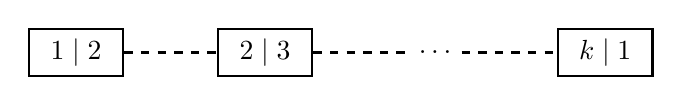
\begin{tikzpicture}[scale=1.2, thick]
  \node[draw, minimum width=1.2cm, minimum height=0.6cm] (D1) at (0,0) {$1 \mid 2$};
  \node[draw, minimum width=1.2cm, minimum height=0.6cm] (D2) at (2,0) {$2 \mid 3$};
  \node (dots) at (3.8,0) {$\dots$};
  \node[draw, minimum width=1.2cm, minimum height=0.6cm] (D3) at (5.6,0) {$k \mid 1$};
  \draw[dashed] (D1) -- (D2);
  \draw[dashed] (D2) -- (dots);
  \draw[dashed] (dots) -- (D3);
\end{tikzpicture}
\end{center}
\end{math-stroke}

\begin{spoken-clean}[00:20:50 - 00:23:00]
Wer hat eine Erklärung dafür? Also wir schauen uns jetzt folgenden Graphen an: Wir nehmen den Graphen $G = (V, E)$, und als Knoten nehmen wir die Zahlen von $0$ bis $16$. Wir haben also diese $17$ Knoten. \inlinemetanote{schreibt an die Tafel}

Und wir sagen, dass zwischen zwei Knoten eine Kante ist, wenn es einen Dominostein gibt. Das sind also unsere Knoten, und die Kanten sind jetzt genau unsere Dominosteine. Okay, jeder Dominostein verbindet ja zwei von diesen Knoten, das macht durchaus Sinn. Wir sagen also, die Kanten --- das sind hier alle Paare $\{a, b\}$, wobei eben $a$ und $b$ in $V$ sind. \inlinemetanote{schreibt an die Tafel}

Okay, jetzt haben wir gesagt, da sehen wir eine gewisse Symmetrie. Wir haben definiert, ein Graph ist regulär vom Grad $n$, wenn jeder Knoten Grad $n$ hat. Das heißt, dieser Graph hier ist regulär vom Grad... wie viel? Ja? $16$? Ja, genau. Wenn man noch die Loops (d.\,h.\ Schlingen) dazu nimmt: $16 + 2 = 18$, genau. Also $18$, weil wenn man eine Zahl hier nimmt, kann man sie zu jeder anderen Zahl verbinden --- das gibt einmal $16$ Kanten, die davon ausgehen, sich selbst ausgenommen. Und dann gibt es aber noch eine Schlinge von dem Knoten zu sich selbst, und das erhöht den Grad um zwei. Das ist zwar nur eine Kante, aber sie geht zurück --- das ist wie mit der person, die sich selbst die Hand schüttelt. Das heißt also $16 + 2 = 18$.
\end{spoken-clean}

\begin{math-stroke}[Modellierung des Dominoproblems]
Wir modellieren das Problem als ungerichteten Graphen $G = (V, E)$ mit:
\begin{itemize}
    \item \textbf{Knotenmenge $V$:} $V := \{0, 1, \dots, 16\}$ (die $17$ Augenzahlen),
    \item \textbf{Kantenmenge $E$:} $E := \{\{a, b\} \mid a, b \in V\}$ (die $153$ Dominosteine).
\end{itemize}
\par\vspace{1ex}\noindent
Dieser Graph $G$ entspricht dem vollständigen Graphen $K_{17}$ mit einer zusätzlichen Schlinge an jedem der $17$ Knoten.
\par\vspace{1ex}\noindent
\textbf{Gradberechnung:} Für jeden Knoten $v \in V$ gilt:
\[
\deg(v) = \underbrace{16}_{\text{Kanten zu anderen Knoten}} + \underbrace{2}_{\text{Schlinge } \{v, v\}} = 18.
\]
Daher ist der Graph $G$ regulär vom Grad $18$.
\end{math-stroke}

\begin{spoken-clean}[00:23:00 - 00:26:34]
Können wir auch hinschreiben, warum das klar ist: $16 + 2$. Das heißt eigentlich --- vom Typ her kann man sagen ---, es ist der vollständige Graph $K_{17}$. Das war der schlichte reguläre Graph vom Grad $16$, bei dem man $17$ Punkte nimmt und jeden Punkt mit jedem anderen verbindet, außer mit sich selbst. Aber hier machen wir einfach an jedem Knoten noch eine Schlinge dran --- also mit $17$ Schlingen dazu. \inlinemetanote{schreibt an die Tafel}

Okay? Und jetzt können wir sagen, daraus folgt: Da der Graph regulär vom Grad $18$ ist, hat jeder Knoten den Grad $18$. Das heißt, es gibt eine geschlossene Euler-Linie. \inlinemetanote{schreibt an die Tafel} Genau, das ist jetzt sozusagen eine Anwendung von dieser eulerschen Charakterisierung auf ein ganz konkretes Problem.

Dasselbe gilt, wenn man andere Dominospiele nimmt: Wenn wir sagen, wir haben andere Augenzahlen, sagen wir, wenn wir nur Zahlen bis $15$ haben, dann geht es natürlich nicht, weil wir dann einen regulären Graphen vom Grad $17$ haben, und dann gibt es keine Lösung mehr. Okay, soweit... soweit klar? \inlinemetanote{Dozent wischt die Tafel und bereitet das nächste Thema vor}
\end{spoken-clean}

\begin{math-stroke}[Lösung des Dominoproblems]
Da $G$ zusammenhängend ist und jeder Knoten einen geraden Grad ($\deg(v) = 18$) besitzt, existiert nach \cref{prop:satz-von-euler} eine geschlossene Euler-Linie.
\par\vspace{1ex}\noindent
\textbf{Antwort:} Ja, es ist möglich, alle Steine zu einer geschlossenen Kette aneinanderzureihen.
\par\vspace{1ex}\noindent
\textbf{Gegenbeispiel (Augenzahlen $0$ bis $15$):} Bei $16$ Augenzahlen wäre der entsprechende Graph $K_{16}$ mit Schlingen regulär vom Grad $15 + 2 = 17$. Da der Grad ungerade ist, existiert keine geschlossene Euler-Linie.
\end{math-stroke}

\begin{spoken-clean}[00:30:15 - 00:31:46]
Gibt es vielleicht noch ein paar Fragezeichen aus dem Publikum? Aber... ja, schauen Sie sich das nochmals an. Das sind eigentlich recht schöne, amüsante Sachen.

Okay, es gibt auch noch ein weiteres Beispiel mit diesen De-Bruijn-Folgen, das können Sie im Skript nachschlagen, wenn Sie das interessiert. Wir gehen weiter zu einem anderen Konzept, das etwas schwieriger ist.

Wir hatten jetzt also Kantenzüge angeschaut, die alle Kanten genau einmal durchlaufen. Jetzt könnten wir uns fragen: Was ist mit einem Kantenzug, der nicht unbedingt alle Kanten einmal durchläuft, aber alle Knoten genau einmal besucht? Und zwar wollen wir einen Kreis, das heißt einen geschlossenen Kantenzug, der jeden Knoten nur einmal enthält. Das ist die folgende Definition.
\end{spoken-clean}

\section{Hamilton-Kreise und Hamilton-Graphen}

\begin{spoken-clean}[00:31:46 - 00:33:32]
Sei $G = (V, E)$ ein ungerichteter, endlicher Graph. Ein Hamilton-Kreis ist ein Kreis in $G$, der alle Knoten von $G$ enthält. Und wir sagen, dass $G$ ein Hamilton-Graph ist, falls $G$ einen Hamilton-Kreis enthält.

Okay, und vielleicht einfach eine Bemerkung hierzu: Es gibt anscheinend kein einfaches Kriterium, um zu entscheiden, ob ein Graph ein Hamilton-Graph ist oder nicht. Das ist also nicht so wie bei Euler-Graphen, bei denen man einfach die Grade aller Knoten anschaut und dann direkt weiß, ob der Graph eulersche Linien besitzt oder nicht. Für Hamilton-Graphen gibt es im Allgemeinen kein einfaches Kriterium. Bei großen Graphen ist das nicht so einfach zu entscheiden, ob es so etwas gibt oder nicht. Aber es gibt durchaus Beispiele, bei denen die Existenz klar ist.
\end{spoken-clean}

\begin{math-stroke}[Definition des Hamilton-Kreises]
\begin{definition}[Hamilton-Kreis und Hamilton-Graph]\label{def:hamilton-kreis}
Sei $G = (V, E)$ ein ungerichteter, endlicher Graph.
\begin{itemize}
    \item Ein \newterm{Hamilton-Kreis} von $G$ ist ein Kreis (d.\,h.\ ein geschlossener Kantenzug ohne Knotenwiederholungen), der sämtliche Knoten von $G$ enthält.
    \item Ein Graph $G$ heißt \newterm{Hamilton-Graph}, wenn er einen Hamilton-Kreis besitzt.
\end{itemize}
\end{definition}
\end{math-stroke}

\begin{spoken-clean}[00:33:32 - 00:35:31]
Also das einfachste Beispiel ist wieder der vollständige Graph $K_n$ ohne Schlingen. Sagen wir, das soll $n \ge 3$ sein --- ich glaube, sogar strikt größer als $2$ ---, dieser ist ein Hamilton-Graph.

Okay, das sieht man ganz einfach: Man beginnt bei $v_1$, man läuft zu irgendeinem anderen Knoten $v_2$. Da wissen wir, dass dieser mit jedem beliebigen anderen Knoten verbunden ist --- es ist ja jeder mit jedem verbunden ---, das heißt, von $v_2$ kann man jetzt zu jedem beliebigen anderen Knoten laufen. Man kann jetzt auf $v_3$ gehen, und so weiter, bis man am Schluss bei $v_n$ anlangt; und von $v_n$ wissen wir, dass er auch wieder mit $v_1$ verbunden ist. Okay, beim vollständigen Graphen $K_n$ ist es also recht einfach.

Dann noch ein Beispiel, das vielleicht noch interessant ist, bei dem man das schön hinzeichnen kann. Ich mache da noch schnell ein Bild davon.

Sie kennen doch die platonischen Körper, oder? Das sind die fünf regulären Polyeder --- also Polyeder, bei denen alle Seitenflächen gleich sind. Und da wissen wir, es gibt genau fünf von diesen: Tetraeder, Würfel, Oktaeder, Dodekaeder und Ikosaeder. Haben Sie wahrscheinlich einmal in der Schule oder sonst wo gesehen. Es lohnt sich, sich das mal anzuschauen. Glauben Sie mir einfach, dass es genau diese fünf gibt.
\end{spoken-clean}

\begin{math-stroke}[Vollständige Graphen als Hamilton-Graphen]
\begin{example}[Vollständiger Graph $K_n$]\label{ex:kn-hamilton}
Der vollständige Graph $K_n$ mit $n \ge 3$ Knoten ist ein Hamilton-Graph.
\end{example}
\begin{short-proof}
Sei $V = \{v_1, v_2, \dots, v_n\}$. Da in $K_n$ alle Paare von Knoten durch eine Kante verbunden sind, existiert der geschlossene Kantenzug:
\[
v_1 \to v_2 \to v_3 \to \dots \to v_n \to v_1
\]
Dieser Kantenzug besucht jeden Knoten genau einmal und kehrt zum Startknoten zurück. Somit ist er ein Hamilton-Kreis.
\end{short-proof}
\end{math-stroke}

\begin{spoken-clean}[00:35:31 - 00:37:58]
Und was wir jetzt machen können: Wir können die Kantengraphen von diesen Körpern anschauen. Das heißt, wir nehmen jetzt einfach... unsere Knoten sind die Ecken von diesen Polyedern, und die Kanten sind die Kanten. Jedem von diesen platonischen Körpern können wir also einen Graphen zuordnen. Da haben wir diese fünf Graphen. Da sehen wir die Knoten und die entsprechenden Kanten dazu --- und die sind alle Hamilton-Graphen.

Wir sehen hier die entsprechenden Kreise: Beim Tetraeder ist das hier der Kantengraph, und dann nehmen wir einfach diesen Kreis hier --- wir sehen, er enthält alle Knoten. Oder beim Würfel können wir den Kantengraph so zeichnen, und da haben wir einen solchen Kreis. Beim Oktaeder sehen wir das auch, wenn man ihn flach auf die Ebene drückt, ist das ein planarer Graph, und da ist es dieser Kreis.

Ja, und Dodekaeder und Ikosaeder sind noch etwas komplizierter, aber man kann sie eigentlich sehr schön darstellen: Man kann sich vorstellen, man nimmt diese Körper, macht einen dieser Kreise ganz groß und drückt den Rest nach innen --- so kann man sie alle schön planar auf der Ebene zeichnen, wenn man möchte. Und da sieht man dann, dass sie alle Hamilton-Graphen sind.

Okay, das wäre also ein weiteres Beispiel für Hamilton-Graphen: die Kantengraphen der fünf platonischen Körper.
\end{spoken-clean}

\begin{math-stroke}[Kantengraphen der platonischen Körper]
\begin{example}[Kantengraphen der platonischen Körper]\label{ex:platonische-koerper}
Die Kantengraphen der fünf platonischen Körper (Tetraeder, Würfel, Oktaeder, Dodekaeder, Ikosaeder) sind Hamilton-Graphen.
\end{example}

\begin{center}
\begin{tabular}{cc}
    \textbf{Tetraeder-Graph} & \textbf{Würfel-Graph ($Q_3$)} \\
    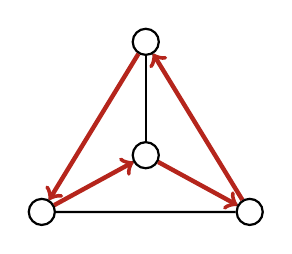
\begin{tikzpicture}[scale=1.2, thick]
      \node[circle, draw, fill=white] (v1) at (0, 1.2) {};
      \node[circle, draw, fill=white] (v2) at (-1.1, -0.6) {};
      \node[circle, draw, fill=white] (v3) at (1.1, -0.6) {};
      \node[circle, draw, fill=white] (v4) at (0, 0) {};
      \draw (v1) -- (v2) -- (v3) -- (v1);
      \draw (v1) -- (v4);
      \draw (v2) -- (v4);
      \draw (v3) -- (v4);
      % Hamilton cycle
      \draw[ultra thick, BrickRed, ->] (v1) -- (v2);
      \draw[ultra thick, BrickRed, ->] (v2) -- (v4);
      \draw[ultra thick, BrickRed, ->] (v4) -- (v3);
      \draw[ultra thick, BrickRed, ->] (v3) -- (v1);
    \end{tikzpicture} &
    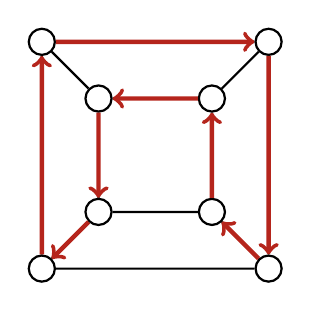
\begin{tikzpicture}[scale=1.2, thick]
      % Outer square
      \node[circle, draw, fill=white] (o1) at (-1.2, 1.2) {};
      \node[circle, draw, fill=white] (o2) at (1.2, 1.2) {};
      \node[circle, draw, fill=white] (o3) at (1.2, -1.2) {};
      \node[circle, draw, fill=white] (o4) at (-1.2, -1.2) {};
      % Inner square
      \node[circle, draw, fill=white] (i1) at (-0.6, 0.6) {};
      \node[circle, draw, fill=white] (i2) at (0.6, 0.6) {};
      \node[circle, draw, fill=white] (i3) at (0.6, -0.6) {};
      \node[circle, draw, fill=white] (i4) at (-0.6, -0.6) {};
      % Connections
      \draw (o1) -- (i1); \draw (o2) -- (i2); \draw (o3) -- (i3); \draw (o4) -- (i4);
      \draw (o1) -- (o2) -- (o3) -- (o4) -- (o1);
      \draw (i1) -- (i2) -- (i3) -- (i4) -- (i1);
      % Hamilton cycle
      \draw[ultra thick, BrickRed, ->] (o1) -- (o2);
      \draw[ultra thick, BrickRed, ->] (o2) -- (o3);
      \draw[ultra thick, BrickRed, ->] (o3) -- (i3);
      \draw[ultra thick, BrickRed, ->] (i3) -- (i2);
      \draw[ultra thick, BrickRed, ->] (i2) -- (i1);
      \draw[ultra thick, BrickRed, ->] (i1) -- (i4);
      \draw[ultra thick, BrickRed, ->] (i4) -- (o4);
      \draw[ultra thick, BrickRed, ->] (o4) -- (o1);
    \end{tikzpicture}
\end{tabular}
\end{center}
\end{math-stroke}

\begin{spoken-clean}[00:37:58 - 00:39:52]
Ein weiteres Beispiel wäre noch der Kantengraph von einem Würfel beliebiger Dimension. Das ist also noch ein weiteres Beispiel: der Kantengraph des $k$-dimensionalen Würfels. Das ist auch ein Hamilton-Graph, und zwar für alle $k \ge \textbf{2}$.

Für $k = 2$ sehen wir: Das ist einfach das Quadrat. Ein zweidimensionaler Würfel ist ein Quadrat, und klar, da kann man einfach einmal rundherumlaufen. Das ist ein Kreis, und das ist ein Hamilton-Kreis, das ist offensichtlich.

Für $k = 3$... Okay, da müssen wir uns auch nicht sehr viel überlegen, das ist auch klar. Da kann man jetzt irgendwie laufen --- was weiß ich, zum Beispiel so: Vielleicht müssen wir eine Farbe nehmen. Man kann irgendwie so laufen, zum Beispiel so, und dann hoch, und dann rüber und nach hinten, und dann so und so und so, und da wieder nach vorne. Wir sehen, das gibt einen Kreis, und alle Knoten werden genau einmal durchlaufen.
\end{spoken-clean}

\begin{math-stroke}[Der $k$-dimensionale Würfel $Q_k$]
\begin{example}[Der $k$-dimensionale Würfel]\label{ex:qk-hamilton}
Der Kantengraph des $k$-dimensionalen Hyperwürfels $Q_k$ ist für alle $k \ge 2$ ein Hamilton-Graph.
\end{example}

\begin{center}
\begin{tikzpicture}[scale=1.4, thick, >=stealth]
  \begin{ai-tikz-planner-invisible-content}
  % 1. Background: 3D-Würfel Q_3 in Kabinett-Projektion mit gestrichelten grauen Kanten für Tiefenwirkung.
  % 2. Foreground: Hamilton-Kreis (Gray-Code) als gerichtete Pfeile (BrickRed, line width=2pt) über die Knoten hinweg gezeichnet.
  % 3. Labels: Eigens positionierte Textknoten mit weißer Füllung gegen Kanten-Kollisionen.
  \end{ai-tikz-planner-invisible-content}

  % Coordinates Front Face
  \coordinate (c000) at (0, 0);
  \coordinate (c100) at (2.5, 0);
  \coordinate (c110) at (2.5, 2.5);
  \coordinate (c010) at (0, 2.5);
  
  % Coordinates Back Face
  \coordinate (c001) at (1.2, 1.0);
  \coordinate (c101) at (3.7, 1.0);
  \coordinate (c111) at (3.7, 3.5);
  \coordinate (c011) at (1.2, 3.5);
  
  % Background / Non-Hamilton Edges (Gray, dashed)
  \draw[gray!50, dashed] (c000) -- (c010);
  \draw[gray!50, dashed] (c100) -- (c101);
  \draw[gray!50, dashed] (c110) -- (c111);
  \draw[gray!50, dashed] (c001) -- (c011);
  
  % Vertices
  \node (nc001) [circle, draw, fill=white, inner sep=2.5pt] at (c001) {};
  \node (nc101) [circle, draw, fill=white, inner sep=2.5pt] at (c101) {};
  \node (nc111) [circle, draw, fill=white, inner sep=2.5pt] at (c111) {};
  \node (nc011) [circle, draw, fill=white, inner sep=2.5pt] at (c011) {};
  
  \node (nc000) [circle, draw, fill=white, inner sep=2.5pt] at (c000) {};
  \node (nc100) [circle, draw, fill=white, inner sep=2.5pt] at (c100) {};
  \node (nc110) [circle, draw, fill=white, inner sep=2.5pt] at (c110) {};
  \node (nc010) [circle, draw, fill=white, inner sep=2.5pt] at (c010) {};
  
  % Hamilton Cycle (BrickRed, bold)
  \draw[->, BrickRed, line width=2pt] (nc010) -- (nc011);
  \draw[->, BrickRed, line width=2pt] (nc011) -- (nc111);
  \draw[->, BrickRed, line width=2pt] (nc111) -- (nc101);
  \draw[->, BrickRed, line width=2pt] (nc101) -- (nc001);
  \draw[->, BrickRed, line width=2pt] (nc001) -- (nc000);
  \draw[->, BrickRed, line width=2pt] (nc000) -- (nc100);
  \draw[->, BrickRed, line width=2pt] (nc100) -- (nc110);
  \draw[->, BrickRed, line width=2pt] (nc110) -- (nc010);
  
  % Labels
  \node[left] at (c000) {\footnotesize $000$};
  \node[right] at (c100) {\footnotesize $100$};
  \node[above right] at (c110) {\footnotesize $110$};
  \node[above left] at (c010) {\footnotesize $010$};
  \node[above left] at (c001) {\footnotesize $001$};
  \node[right] at (c101) {\footnotesize $101$};
  \node[above right] at (c111) {\footnotesize $111$};
  \node[above] at (c011) {\footnotesize $011$};
\end{tikzpicture}
\end{center}
\end{math-stroke}

\begin{spoken-clean}[00:39:52 - 00:41:53]
Okay, und für beliebiges $k$ müssen wir uns das wie folgt vorstellen: Wir schauen uns jetzt den $k$-dimensionalen Würfel an. Wir betrachten im $\mathbb{R}^k$ all die Punkte --- die Knoten sind genau die Punkte, bei denen alle Koordinaten aus Nullen und Einsen bestehen.

Und zwei davon sind genau dann verbunden, wenn sie sich in genau einer Stelle unterscheiden. Das ist unser Würfel. Das heißt, wir identifizieren die... wie viele Ecken hat eigentlich ein $k$-dimensionaler Würfel? Ja?
\end{spoken-clean}

\begin{student-interaction}[Student Answer]
$2^k$.
\end{student-interaction}

\begin{spoken-clean}[00:39:52 - 00:41:53]
$2^k$, genau. Wir identifizieren die $2^k$ Ecken des $k$-dimensionalen Würfels mit binären Wörtern der Länge $k$. Was ist ein binäres Wort? Das ist einfach ein Wort bestehend aus Nullen und Einsen --- also die Elemente in $\{0, 1\}^k$.

Und zwei solche Wörter $a$ und $b$ sind durch eine Kante verbunden, falls sie sich in genau einer Stelle unterscheiden. Okay. Und wir schauen uns dann nach der Pause an, weshalb daraus folgt beziehungsweise weshalb das zeigt, dass es immer einen Hamilton-Kreis im $k$-dimensionalen Würfel gibt. Gut, wir machen in einer Viertelstunde weiter.
\end{spoken-clean}

\begin{math-stroke}[Formale Definition des $k$-dimensionalen Würfels]
\begin{definition}[$k$-dimensionaler Würfel $Q_k$]\label{def:qk-formal}
Der \newterm{$k$-dimensionale Würfel} $Q_k$ ist der ungerichtete Graph $G = (V, E)$ mit:
\begin{itemize}
    \item \textbf{Knotenmenge $V$:} $V := \{0, 1\}^k$ (die Menge aller binären Wörter der Länge $k$),
    \item \textbf{Kantenmenge $E$:} $E := \{\{a, b\} \mid a, b \in V \text{ mit } d_H(a, b) = 1\}$, wobei $d_H(a, b)$ den Hamming-Abstand bezeichnet (die Anzahl der Stellen, in denen sich $a$ and $b$ unterscheiden).
\end{itemize}
\end{definition}
\end{math-stroke}

\begin{lecture-break}[Vorlesungspause]
Der Dozent kündigt eine 15-minütige Pause an. Das Video wird nach der Pause bei Zeitstempel 00:14:22 fortgesetzt.
\end{lecture-break}

\begin{spoken-clean}[00:43:56 - 00:46:03]
Also, wir haben hier unseren $k$-dimensionalen Würfel. Und wir wollen zeigen, dass dieser Kantengraph hier ein Hamilton-Graph ist. Das folgt aus der folgenden Behauptung, die wir beweisen werden. Was sagt diese Behauptung? Sie sagt:

Es gibt eine zyklische Folge --- nennen wir sie $a_1$ bis $a_{2^k}$ --- aus den $2^k$ verschiedenen binären Wörtern der Länge $k$, sodass sich $a_\ell$ und $a_{\ell+1}$ für $\ell = 1$ bis $2^k - 1$ sowie $a_{2^k}$ und $a_1$ in genau einer Stelle unterscheiden.

Wir müssen also zeigen, dass eine solche Folge existiert, bei der wir immer nur ein Bit wechseln und am Schluss wieder am Anfang ankommen. Eine solche Folge nennt man einen Gray-Code.
\end{spoken-clean}

\begin{math-stroke}[Existenz eines Gray-Codes]
\begin{proposition}[Existenz eines Gray-Codes]\label{prop:gray-code-existenz}
Für jedes $k \in \mathbb{N}_{>0}$ existiert eine zyklische Folge $(a_1, a_2, \dots, a_{2^k})$ aller $2^k$ binären Wörter der Länge $k$, sodass sich aufeinanderfolgende Wörter (sowie das letzte und das erste Wort) in genau einer Stelle unterscheiden:
\begin{itemize}
    \item $d_H(a_\ell, a_{\ell+1}) = 1 \quad \forall \ell \in \{1, \dots, 2^k-1\}$,
    \item $d_H(a_{2^k}, a_1) = 1$.
\end{itemize}
Eine solche Folge heißt \newterm{Gray-Code} $k$-ter Ordnung.
\end{proposition}
\end{math-stroke}

\begin{spoken-clean}[00:46:03 - 00:48:21]
Okay. Ich weiß nicht Genaueres darüber, weshalb das Gray-Code heißt. Das kommt wahrscheinlich aus der Codierungstheorie, in der man untersucht, wie man Wörter gut wählt, um Informationen verlässlich zu übermitteln --- fehlerkorrigierende Codes und so weiter. Aber das ist für uns nicht so wichtig; wichtig ist für uns nur zu beweisen, dass es eine solche Folge immer gibt.

Und der Beweis ist nicht schwierig, das ist einfach Induktion nach $k$. Für $k = 1$ ist die Sache klar: Bei Wörtern der Länge $1$ nehmen wir einfach die Folge $(0, 1)$. $1$ unterscheidet sich in einer Stelle von $0$, und $0$ unterscheidet sich in einer Stelle von $1$.

Um anschließend von $k$ auf $k+1$ zu schließen, nehmen wir an, es gibt einen Gray-Code $k$-ter Ordnung --- das sei die Folge $(a_1, a_2, \dots, a_{2^k})$. Daraus können wir jetzt ganz einfach einen Gray-Code für $k+1$ bauen.

Und zwar machen wir das so: Wir hängen zuerst überall eine $0$ vorne an, also machen wir $0a_1, 0a_2, \dots, 0a_{2^k}$. Diese unterscheiden sich untereinander jeweils nur in einer Stelle, da sich die $a_i$ jeweils nur in einer Stelle unterscheiden.

Und jetzt machen wir am Übergang mit $1a_{2^k}$ weiter. Diese beiden ($0a_{2^k}$ und $1a_{2^k}$) unterscheiden sich auch wieder nur in einer Stelle, nämlich in der ersten. Und jetzt gehen wir einfach die Folge rückwärts zurück, bis wir bei $1a_1$ angelangt sind. Das ist dann offensichtlich auch wieder ein Gray-Code. Und ein solcher Gray-Code entspricht natürlich genau einem Hamilton-Kreis auf dem Kantengraphen des Würfels.
\end{spoken-clean}

\begin{math-stroke}[Beweis der Existenz von Gray-Codes]
\begin{short-proof}[Beweis von \cref{prop:gray-code-existenz}]
Wir führen den Beweis mittels vollständiger Induktion nach $k \in \mathbb{N}_{>0}$:
\begin{itemize}
    \item \textbf{Induktionsanfang ($k=1$):}
    Die Folge $(0, 1)$ ist ein Gray-Code der Ordnung $1$, da $d_H(0, 1) = 1$ and $d_H(1, 0) = 1$.
    \item \textbf{Induktionsschritt ($k \to k+1$):}
    Sei $(a_1, a_2, \dots, a_{2^k})$ ein Gray-Code $k$-ter Ordnung. Wir konstruieren eine Folge für $k+1$ durch Spiegelung und Präfix-Erweiterung:
    \[
    (0a_1, 0a_2, \dots, 0a_{2^k}, 1a_{2^k}, 1a_{2^k-1}, \dots, 1a_1)
    \]
    \textbf{Verifikation der Hamming-Abstände:}
    \begin{itemize}
        \item Für die erste Hälfte gilt $d_H(0a_\ell, 0a_\ell+1) = d_H(a_\ell, a_\ell+1) = 1$ nach Induktionsvoraussetzung.
        \item Am Übergangspunkt gilt $d_H(0a_{2^k}, 1a_{2^k}) = 1$ (Unterschied nur im ersten Bit).
        \item Für die gespiegelte zweite Hälfte gilt analog $d_H(1a_\ell, 1a_{\ell-1}) = 1$.
        \item Am Rückkehrpunkt gilt $d_H(1a_1, 0a_1) = 1$.
    \end{itemize}
    Somit ist die konstruierte Folge ein gültiger Gray-Code der Ordnung $k+1$.
\end{itemize}
\end{short-proof}
\end{math-stroke}

\section{Bipartite Graphen und der Heiratssatz}
\subsection{Definition und Eigenschaften}

\begin{spoken-clean}[00:54:05 - 00:55:02]
Als letztes Thema möchte ich heute noch den sogenannten Heiratssatz besprechen, obwohl das ein sehr unglücklicher Name ist. Zuvor noch eine Definition, die auch auf dem Übungsblatt vorkommt: Ein Graph heißt bipartit. Bipartit ist ein lustiges Wort. Was heißt das? Man kann den Graphen in zwei Teile teilen, also man kann die Knotenmenge in zwei verschiedene Mengen aufteilen, sodass alle Kanten ausschließlich zwischen der einen Menge und der anderen Menge verlaufen.

Er heißt also bipartit, falls $V$ die disjunkte Vereinigung von zwei Teilmengen $U$ und $W$ ist --- disjunkte Vereinigung (geschrieben als $U \;\dot{\cup}\; W$) bedeutet, dass $V = U \cup W$ ist und der Durchschnitt $U \cap W = \emptyset$ leer ist ---, sodass die Kanten alle in der Menge $U \times W$ enthalten sind (d.\,h.\ $E \subseteq \{\{u, w\} \mid u \in U, w \in W\}$). Wir schreiben den Graphen dann einfach als $G = (U, W, E)$.

Okay, wenn wir sagen, $G$ ist ein bipartiter Graph und wir schreiben ihn so, dann heißt das: Das eine ist die eine Knotenmenge, das andere die andere, und die Kanten gehen alle von Elementen hier zu Elementen da. Es gibt natürlich Graphen, die nicht bipartit sind --- das ist eine sehr spezielle Klasse von Graphen, die meisten sind es nicht. Es gibt dazu noch eine Übungsaufgabe, in der wir uns eine Verallgemeinerung davon anschauen, nämlich die Frage, wie ein Graph färbbar ist. Ein Graph ist genau dann bipartit, wenn er zweifärbbar ist. Das heißt, man kann allen Knoten eine Farbe --- blau oder rot --- geben, sodass nie zwei gleichfarbige Knoten durch eine Kante verbunden sind (d.\,h.\ es geht nie eine Kante von einem roten Knoten zu einem roten Knoten, sondern immer nur zu einem blauen). Gut, okay, das sind bipartite Graphen.
\end{spoken-clean}

\begin{math-stroke}[Bipartite Graphen]
\begin{definition}[Bipartiter Graph]\label{def:bipartiter-graph}
Ein Graph $G = (V, E)$ heißt \newterm{bipartit}, wenn sich seine Knotenmenge $V$ als disjunkte Vereinigung zweier Teilmengen $U$ und $W$ darstellen lässt:
\[
V = U \;\dot{\cup}\; W \quad (\text{d.\,h.\ } V = U \cup W \text{ und } U \cap W = \emptyset),
\]
sodass alle Kanten $e \in E$ ausschließlich Knoten aus $U$ mit Knoten aus $W$ verbinden:
\[
E \subseteq \{ \{u, w\} \mid u \in U, \ w \in W \}.
\]
Wir schreiben dafür auch $G = (U, W, E)$.
\end{definition}

\begin{center}
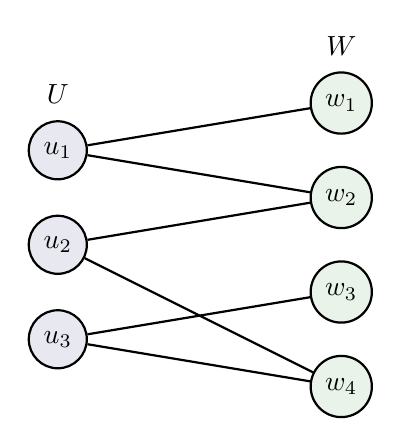
\begin{tikzpicture}[scale=1.2, thick, >=stealth]
  % Set U (left)
  \node[circle, draw, fill=MidnightBlue!10] (u1) at (0, 2) {$u_1$};
  \node[circle, draw, fill=MidnightBlue!10] (u2) at (0, 1) {$u_2$};
  \node[circle, draw, fill=MidnightBlue!10] (u3) at (0, 0) {$u_3$};
  \node at (0, 2.6) {\textbf{$U$}};

  % Set W (right)
  \node[circle, draw, fill=ForestGreen!10] (w1) at (3, 2.5) {$w_1$};
  \node[circle, draw, fill=ForestGreen!10] (w2) at (3, 1.5) {$w_2$};
  \node[circle, draw, fill=ForestGreen!10] (w3) at (3, 0.5) {$w_3$};
  \node[circle, draw, fill=ForestGreen!10] (w4) at (3, -0.5) {$w_4$};
  \node at (3, 3.1) {\textbf{$W$}};

  % Edges between U and W
  \draw (u1) -- (w1);
  \draw (u1) -- (w2);
  \draw (u2) -- (w2);
  \draw (u2) -- (w4);
  \draw (u3) -- (w3);
  \draw (u3) -- (w4);
\end{tikzpicture}
\end{center}
\end{math-stroke}

\subsection{Nachbarschaftsmengen in bipartiten Graphen}

\begin{spoken-clean}[00:55:02 - 00:56:41]
Das heißt, bei bipartiten Graphen spielt es oft keine so große Rolle mehr, ob sie gerichtet oder ungerichtet sind. Man weiß eigentlich für jede Kante genau, ob sie in $U$ anfängt und in $W$ aufhört, selbst wenn der Graph ungerichtet ist.
\end{spoken-clean}

\begin{spoken-clean}[00:56:41 - 00:59:04]
Bipartite Graphen treten natürlich in der Praxis relativ häufig auf. Was weiß ich, wenn man zum Beispiel Brieffreunde zwischen Europa und Amerika betrachtet: Die Personen sind entweder in Europa oder in Amerika ansässig, aber sie schreiben sich Briefe nur über den Atlantik hinweg. Das wäre ein klassischer bipartiter Graph.

Okay, machen wir noch eine Definition --- das ist eigentlich eher für ungerichtete Graphen. Für einen ungerichteten bipartiten Graphen $G = (U, W, E)$ definieren wir für eine Teilmenge $X \subseteq U$ die Nachbarschaftsmenge $E(X)$ als die Menge aller $y \in W$, für die ein $x \in X$ existiert, sodass $\{x, y\} \in E$ eine Kante ist. Und ganz ähnlich definieren wir auch $E(Y)$ für eine Teilmenge $Y \subseteq W$.
\end{spoken-clean}

\begin{math-stroke}[Nachbarschaftsmengen in bipartiten Graphen]
\begin{definition}[Nachbarschaftsmenge]\label{def:nachbarschaftsmenge}
Sei $G = (U, W, E)$ ein ungerichteter, bipartiter Graph. Für eine Teilmenge $X \subseteq U$ definieren wir die Nachbarschaftsmenge $E(X) \subseteq W$ durch:
\[
E(X) := \{ y \in W \mid \exists x \in X \colon \{x, y\} \in E \}.
\]
Analog definieren wir für eine Teilmenge $Y \subseteq W$ die Nachbarschaftsmenge $E(Y) \subseteq U$.
\end{definition}
\end{math-stroke}

\begin{math-stroke}[Geometrische Veranschaulichung der Nachbarschaftsmenge]
\begin{center}
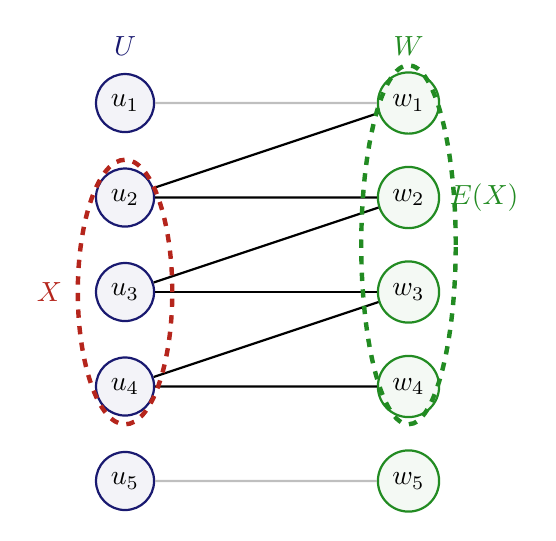
\begin{tikzpicture}[scale=1.2, >=stealth, thick]
  % [AI-TIKZ-PLANNER: Bipartite Graph Neighborhood E(X)]
  % 1. Background: Left column U (blue) and right column W (green).
  % 2. Midground: Circle subset X in U and its corresponding neighborhood E(X) in W.
  % 3. Foreground: Edges connecting elements of X to E(X), plus some outside edges.
  
  % Left column (U)
  \node[circle, draw=MidnightBlue, fill=MidnightBlue!5, minimum size=0.6cm] (u1) at (0, 2) {$u_1$};
  \node[circle, draw=MidnightBlue, fill=MidnightBlue!5, minimum size=0.6cm] (u2) at (0, 1) {$u_2$};
  \node[circle, draw=MidnightBlue, fill=MidnightBlue!5, minimum size=0.6cm] (u3) at (0, 0) {$u_3$};
  \node[circle, draw=MidnightBlue, fill=MidnightBlue!5, minimum size=0.6cm] (u4) at (0, -1) {$u_4$};
  \node[circle, draw=MidnightBlue, fill=MidnightBlue!5, minimum size=0.6cm] (u5) at (0, -2) {$u_5$};
  \node[MidnightBlue] at (0, 2.6) {\textbf{$U$}};

  % Right column (W)
  \node[circle, draw=ForestGreen, fill=ForestGreen!5, minimum size=0.6cm] (w1) at (3, 2) {$w_1$};
  \node[circle, draw=ForestGreen, fill=ForestGreen!5, minimum size=0.6cm] (w2) at (3, 1) {$w_2$};
  \node[circle, draw=ForestGreen, fill=ForestGreen!5, minimum size=0.6cm] (w3) at (3, 0) {$w_3$};
  \node[circle, draw=ForestGreen, fill=ForestGreen!5, minimum size=0.6cm] (w4) at (3, -1) {$w_4$};
  \node[circle, draw=ForestGreen, fill=ForestGreen!5, minimum size=0.6cm] (w5) at (3, -2) {$w_5$};
  \node[ForestGreen] at (3, 2.6) {\textbf{$W$}};

  % Edges
  \draw[gray!50] (u1) -- (w1);
  \draw[thick] (u2) -- (w1);
  \draw[thick] (u2) -- (w2);
  \draw[thick] (u3) -- (w2);
  \draw[thick] (u3) -- (w3);
  \draw[thick] (u4) -- (w3);
  \draw[thick] (u4) -- (w4);
  \draw[gray!50] (u5) -- (w5);

  % Circle subset X (BrickRed)
  \draw[dashed, BrickRed, ultra thick] (0, 0) ellipse (0.5cm and 1.4cm);
  \node[BrickRed] at (-0.8, 0) {\textbf{$X$}};

  % Circle subset E(X) (ForestGreen)
  \draw[dashed, ForestGreen, ultra thick] (3, 0.5) ellipse (0.5cm and 1.9cm);
  \node[ForestGreen] at (3.8, 1) {\textbf{$E(X)$}};
\end{tikzpicture}
\end{center}

\begin{explanation-of-steps}[Bedeutung der Nachbarschaftsmenge]
Die Nachbarschaftsmenge $E(X)$ (auch als \newterm{Schnitt} oder \newterm{Kantenbild} bezeichnet) besteht aus allen Knoten der Partition $W$, die über mindestens eine Kante mit einem Knoten aus der Teilmenge $X \subseteq U$ verbunden sind.
\end{explanation-of-steps}
\end{math-stroke}

\begin{spoken-clean}[00:56:47 - 00:58:37]
Bipartit heißt also: Hier drüben haben wir alle Knoten aus $U$, dort drüben alle Knoten aus $W$. \inlinemetanote{zeigt auf die Zeichnung an der Tafel} Und gewisse davon sind miteinander verbunden --- was weiß ich, ein ganz normaler Graph eben.

Wenn wir jetzt hier eine Teilmenge von $U$ haben, sagen wir $X$ zum Beispiel, dann schauen wir uns das $E(X)$ an. Das sind dann alle Knoten in $W$, die mit mindestens einem Knoten in $X$ verbunden sind. Und ganz ähnlich definieren wir auch $E(Y)$ für eine Teilmenge $Y \subseteq W$.

Es geht hierbei um das folgende Problem, das ich kurz erklären möchte. \inlinemetanote{wischt die mittlere Tafel}
\end{spoken-clean}

\subsection{Der Heiratssatz von Hall}

\begin{spoken-clean}[00:58:37 - 01:01:27]
Ich sage jetzt schon gar nicht, weshalb das \qt{Heiratssatz} heißt, weil das auf vollständig veralteten, chauvinistischen, heteronormativen, monogamen Definitionen von Heirat und sehr binären Geschlechtsdefinitionen beruht. Das wollen wir uns gar nicht erst anschauen. Aber es ist eben ein Satz aus den 30er-Jahren (Philip Hall, 1935).

Ich kann das Problem aber anders erklären, sagen wir als Geschenkeverteilung. Wir haben folgendes Problem: Hier haben wir Kinder, $A, B, C, D, E$ zum Beispiel. Und dort drüben gibt es Geschenke, $1, 2, 3, 4, 5, 6$, die diese Kinder gerne hätten. Jede dieser Personen hat gewisse Präferenzen: Zum Beispiel möchte $A$ gerne Geschenk $1$ oder $3$, $B$ möchte gerne $2, 4, 5$ oder $6$, $C$ möchte gerne $2$ oder $3$, $D$ möchte $1$ oder $4$, und so weiter.

Das kennt man ja vom Kindergeburtstag: Jeder darf sich ein Geschenk aus dem Korb aussuchen, und jedes Kind hat vielleicht drei, vier Sachen, die es gerne hätte. Gibt es eine Möglichkeit, die Geschenke so zu verteilen, dass jedes Kind ein Geschenk bekommt, das es sich auch gewünscht hat?

Die mathematische Frage lautet also: Gibt es eine injektive Funktion von dieser Menge $U$ (Kinder) zu jener Menge $W$ (Geschenke)? Wir wollen jedem Kind ein Geschenk zuordnen, allerdings unter der Bedingung, dass wir ein Kind nur mit einem Geschenk paaren dürfen, das im Graphen durch eine Kante verbunden ist (d.\,h.\ das auf der Präferenzliste steht). Das ist ein sehr klassisches Alltagsproblem --- vor allem bei großen Gruppen von Kindern und Geschenken. Es kann aber natürlich auch in vielen anderen Kontexten eine Rolle spielen, zum Beispiel bei der Zuweisung von Betreuerinnen für Masterarbeiten.

Und die Frage ist: Wann hat dieses Problem eine Lösung? Für welche Graphen gibt es eine solche Injektion?
\end{spoken-clean}

\begin{math-stroke}[Das Heiratsproblem als bipartiter Graph]
\begin{center}
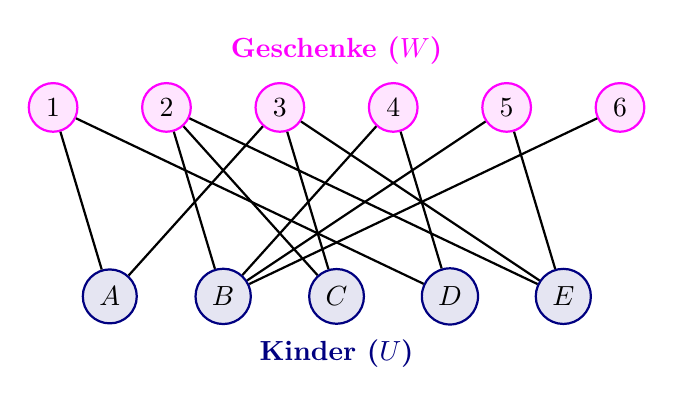
\begin{tikzpicture}[scale=1.2, thick]
  % [AI-TIKZ-PLANNER: Marriage Theorem Example (Gifts and Children)]
  % 1. Background: Top row of gifts (pink) and bottom row of children (blue).
  % 2. Foreground: Edges representing preferences.
  
  % Top row (Gifts)
  \node[circle, draw=Fuchsia, fill=Fuchsia!10, minimum size=0.6cm] (g1) at (0, 2) {$1$};
  \node[circle, draw=Fuchsia, fill=Fuchsia!10, minimum size=0.6cm] (g2) at (1.2, 2) {$2$};
  \node[circle, draw=Fuchsia, fill=Fuchsia!10, minimum size=0.6cm] (g3) at (2.4, 2) {$3$};
  \node[circle, draw=Fuchsia, fill=Fuchsia!10, minimum size=0.6cm] (g4) at (3.6, 2) {$4$};
  \node[circle, draw=Fuchsia, fill=Fuchsia!10, minimum size=0.6cm] (g5) at (4.8, 2) {$5$};
  \node[circle, draw=Fuchsia, fill=Fuchsia!10, minimum size=0.6cm] (g6) at (6.0, 2) {$6$};
  \node[Fuchsia] at (3.0, 2.6) {\textbf{Geschenke ($W$)}};

  % Bottom row (Children)
  \node[circle, draw=NavyBlue, fill=NavyBlue!10, minimum size=0.6cm] (cA) at (0.6, 0) {$A$};
  \node[circle, draw=NavyBlue, fill=NavyBlue!10, minimum size=0.6cm] (cB) at (1.8, 0) {$B$};
  \node[circle, draw=NavyBlue, fill=NavyBlue!10, minimum size=0.6cm] (cC) at (3.0, 0) {$C$};
  \node[circle, draw=NavyBlue, fill=NavyBlue!10, minimum size=0.6cm] (cD) at (4.2, 0) {$D$};
  \node[circle, draw=NavyBlue, fill=NavyBlue!10, minimum size=0.6cm] (cE) at (5.4, 0) {$E$};
  \node[NavyBlue] at (3.0, -0.6) {\textbf{Kinder ($U$)}};

  % Edges (Preferences)
  \draw (cA) -- (g1); \draw (cA) -- (g3);
  \draw (cB) -- (g2); \draw (cB) -- (g4); \draw (cB) -- (g5); \draw (cB) -- (g6);
  \draw (cC) -- (g2); \draw (cC) -- (g3);
  \draw (cD) -- (g1); \draw (cD) -- (g4);
  \draw (cE) -- (g2); \draw (cE) -- (g3); \draw (cE) -- (g5);
\end{tikzpicture}
\end{center}

\begin{explanation-of-steps}[Mathematische Formulierung]
Das Problem besteht darin, eine injektive Auswahlfunktion (ein \newterm{Matching}) $\pi \colon U \to W$ zu finden, sodass für jedes Kind $u \in U$ das zugeordnete Geschenk $\pi(u) \in W$ in seiner Präferenzmenge liegt, d.\,h.\ $\{u, \pi(u)\} \in E$.
\end{explanation-of-steps}
\end{math-stroke}

\begin{spoken-clean}[01:01:27 - 01:04:12]
Der Heiratssatz gibt uns eine notwendige und hinreichende Bedingung. Denn wenn natürlich alle Kinder dasselbe Geschenk wollen, kann es keine solche Injektion geben, das ist völlig klar.

Der Heiratssatz von Philip Hall --- einem bekannten Gruppentheoretiker --- besagt Folgendes: Sei $G = (V, E)$ ein endlicher, ungerichteter, bipartiter Graph. Dann sind die folgenden Aussagen äquivalent: \inlinemetanote{schreibt an die Tafel}

\textbf{(a)} Es existiert eine Injektion $\pi \colon A \to B$, sodass für alle $a \in A$ gilt: $\{a, \pi(a)\} \in E$ (d.\,h.\ das zugeordnete Element ist durch eine Kante verbunden).

\textbf{(b)} Für alle Teilmengen $X \subseteq A$ gilt die Hall-Bedingung: $|X| \le |E(X)|$.

Manche Leute formulieren das anschaulich so: Zwei Elemente $a \in A$ und $b \in B$ heißen befreundet, falls eine Kante $\{a, b\} \in E$ existiert. Eine solche Injektion $\pi$ nennt man dann eine \qt{Heiratsfunktion}. Die Frage ist also: Kann man alle Elemente von $A$ monogam mit Elementen von $B$ verheiraten, sodass nur befreundete Paare verheiratet werden? Und diese Hall-Bedingung ist dafür sowohl notwendig als auch hinreichend.
\end{spoken-clean}

\begin{math-stroke}[Der Heiratssatz von Hall]
\begin{theorem}[Heiratssatz von Hall]\label{thm:heiratssatz-hall}
Sei $G = (A, B, E)$ ein endlicher, ungerichteter, bipartiter Graph. Dann sind die folgenden Aussagen äquivalent:
\begin{enumerate}[label=\textbf{(\alph*)}]
    \item Es existiert eine Injektion $\pi \colon A \to B$, sodass für alle $a \in A$ gilt:
    \[
    \{a, \pi(a)\} \in E.
    \]
    \item Für alle Teilmengen $X \subseteq A$ gilt die \newterm{Hall-Bedingung}:
    \begin{equation}\label{eq:hall-bedingung}
    |X| \le |E(X)|.
    \end{equation}
\end{enumerate}
\end{theorem}
\end{math-stroke}

\begin{proof}[Beweis des Heiratssatzes von Hall]

\begin{spoken-clean}[01:04:12 - 01:06:32]
Kommen wir zum Beweis. \inlinemetanote{schreibt an die Tafel}

Die Richtung \textbf{(a)} $\implies$ \textbf{(b)} ist relativ klar: Wenn wir wissen, dass eine solche Injektion $\pi$ existiert, dann ist für jede Teilmenge $X \subseteq A$ die Kardinalität $|X|$ gleich der Kardinalität des Bildes $|\pi(X)|$. Da alle Elemente im Bild $\pi(X)$ über Kanten mit Elementen aus $X$ verbunden sind, ist dieses Bild eine Teilmenge der Nachbarschaftsmenge $E(X)$. Daraus folgt sofort: $|X| = |\pi(X)| \le |E(X)|$. Und das gilt für alle Teilmengen $X \subseteq A$. Es ist also offensichtlich, dass die Bedingung notwendig ist.

Der eigentlich interessante Teil des Satzes ist die Rückrichtung \textbf{(b)} $\implies$ \textbf{(a)}, also dass die Bedingung auch hinreichend ist. Wir beweisen dies per vollständiger Induktion nach der Anzahl der Elemente in $A$ (d.\,h.\ nach $n = |A|$). \inlinemetanote{schreibt an die Tafel}

Wir nehmen an, die Aussage sei für alle Graphen mit $|A| = n$ bereits bewiesen, und wollen sie nun für $|A| = n+1$ zeigen. Dazu unterscheiden wir zwei Fälle.
\end{spoken-clean}

\begin{math-stroke}[Beweis der Notwendigkeit und Induktionsanfang]
\begin{short-proof}[Hinrichtung \texorpdfstring{$\mathbf{(a) \implies (b)}$}{(a) => (b)}]
Sei $\pi \colon A \to B$ eine Injektion mit $\{a, \pi(a)\} \in E$ für alle $a \in A$. Für eine beliebige Teilmenge $X \subseteq A$ gilt aufgrund der Injektivität von $\pi$:
\[
|X| = |\pi(X)|.
\]
Da für jedes $x \in X$ gilt, dass $\pi(x) \in E(X)$ (da $\{x, \pi(x)\} \in E$), folgt $\pi(X) \subseteq E(X)$. Somit gilt:
\[
|X| = |\pi(X)| \le |E(X)|.
\]
Dies zeigt die Notwendigkeit der Hall-Bedingung.
\end{short-proof}

\begin{short-proof}[Rückrichtung \texorpdfstring{$\mathbf{(b) \implies (a)}$}{(b) => (a)} --- Induktionsanfang]
Wir führen den Beweis mittels vollständiger Induktion nach $n = |A|$:
\par\vspace{1ex}\noindent
\textbf{Induktionsanfang ($n = 1$):} Sei $A = \{a_1\}$. Die Bedingung \eqref{eq:hall-bedingung} für $X = A$ liefert:
\[
1 = |A| \le |E(A)| \implies |E(A)| \ge 1.
\]
Es existiert also mindestens ein $b_1 \in B$ mit $\{a_1, b_1\} \in E$. Die Abbildung $\pi(a_1) := b_1$ ist eine wohldefinierte Injektion.
\end{short-proof}
\end{math-stroke}

\subsubsection{Induktionsschritt: Fall 1}

\begin{spoken-clean}[01:06:32 - 01:08:47]
\textbf{Fall 1:} Für alle echten Teilmengen $\emptyset \neq X \subsetneq A$ gilt die strikte Ungleichung $|X| < |E(X)|$.

Die Hall-Bedingung sagt uns im Allgemeinen nur, dass $|X| \le |E(X)|$ ist. In diesem ersten Fall nehmen wir aber an, dass für jede echte Teilmenge sogar die strikte Ungleichung gilt.

In diesem Fall wählen wir eine beliebige Kante $\{a', b'\} \in E$. Wir betrachten nun die reduzierten Mengen $A' := A \setminus \{a'\}$ und $B' := B \setminus \{b'\}$ sowie die induzierte Kantenmenge $E'$, die alle Kanten aus $E$ enthält, die zwischen $A'$ und $B'$ verlaufen. Das sind genau die Kanten, die weder mit $a'$ noch mit $b'$ inzident sind.
\end{spoken-clean}

\begin{spoken-clean}[01:08:47 - 01:10:52]
Wenn wir jetzt irgendeine Teilmenge $X \subseteq A'$ betrachten, dann ist $X$ auch eine echte Teilmenge von $A$. Nach unserer Fall-1-Annahme gilt also $|X| < |E(X)|$. Daraus folgt direkt: $|X| \le |E(X)| - 1$.

Da $E'(X)$ mindestens alle Nachbarn aus $E(X)$ außer eventuell $b'$ enthält, gilt $|E'(X)| \ge |E(X) \setminus \{b'\}| \ge |E(X)| - 1 \ge |X|$. Schlimmstenfalls verlieren wir durch das Weglassen von $b'$ also nur einen Nachbarn, sodass die Hall-Bedingung für den reduzierten Graphen immer noch erfüllt bleibt.

Das bedeutet, dass der reduzierte Graph $G' = (A', B', E')$ die Hall-Bedingung ebenfalls erfüllt. Da $|A'| = n$ ist, existiert nach Induktionsvoraussetzung eine Injektion $\pi' \colon A' \to B'$ mit $\{a, \pi'(a)\} \in E'$ für alle $a \in A'$.

Wir können diese Abbildung nun zu einer Funktion $\pi \colon A \to B$ fortsetzen, indem wir definieren: $\pi(a) := b'$, falls $a = a'$ ist, und $\pi(a) := \pi'(a)$ andernfalls. Diese Abbildung ist offensichtlich injektiv und erfüllt die Bedingung \textbf{(a)} für den gesamten Graphen.
\end{spoken-clean}

\begin{math-stroke}[Induktionsschritt: Fall 1]
\begin{short-proof}[Beweis von Fall 1]
\textbf{Fall 1: Strikte Ungleichung für alle echten Teilmengen.}
Es gelte $|X| < |E(X)|$ für alle echten Teilmengen $\emptyset \neq X \subsetneq A$.
\par\vspace{1ex}\noindent
Wähle eine beliebige Kante $\{a', b'\} \in E$. Wir definieren den reduzierten Graphen $G' = (A', B', E')$ durch:
\begin{align*}
A' &:= A \setminus \{a'\} \\
B' &:= B \setminus \{b'\} \\
E' &:= E \cap (A' \times B')
\end{align*}
Für jede Teilmenge $X \subseteq A'$ gilt, da $X$ eine echte Teilmenge von $A$ ist ($|X| < |A|$):
\[
|X| \le |E(X)| - 1.
\]
Da $E'(X) \ge E(X) \setminus \{b'\}$, folgt:
\[
|E'(X)| \ge |E(X)| - 1 \ge |X|.
\]
Somit erfüllt der Teilgraph $G'$ die Hall-Bedingung. Nach Induktionsvoraussetzung existiert eine Injektion $\pi' \colon A' \to B'$ mit $\{a, \pi'(a)\} \in E'$ für alle $a \in A'$.
\par\vspace{1ex}\noindent
Wir definieren die Abbildung $\pi \colon A \to B$ durch:
\[
\pi(a) := \begin{cases}
b' & \text{falls } a = a' \\
\pi'(a) & \text{falls } a \in A'
\end{cases}
\]
Diese Abbildung $\pi$ ist injektiv und erfüllt $\{a, \pi(a)\} \in E$ für alle $a \in A$.
\end{short-proof}
\end{math-stroke}

\subsubsection{Induktionsschritt: Fall 2}

\begin{spoken-clean}[01:10:52 - 01:12:42]
Okay, dieser erste Fall ist also relativ klar: Wir haben unsere Knoten in $A$ und unsere Knoten in $B$. Wir nehmen einfach eine Kante heraus, und dank der starken Fall-1-Bedingung erfüllt der verbleibende Teilgraph immer noch die Hall-Bedingung. Wir erhalten per Induktion eine Injektion für den Rest und setzen diese durch die herausgenommene Kante fort. Soweit, so gut.

Schauen wir uns nun \textbf{Fall 2} an: Wir befinden uns nicht im ersten Fall. Das heißt, es gilt nicht für alle echten Teilmengen $X \subsetneq A$, dass $|X| < |E(X)|$ ist. Da die Hall-Bedingung für den Gesamtgraphen gilt, bedeutet dies, dass eine echte Teilmenge $\emptyset \neq A_1 \subsetneq A$ existiert, für die Gleichheit gilt:
\[
|A_1| = |E(A_1)|.
\]
\end{spoken-clean}

\begin{spoken-clean}[01:12:42 - 01:15:02]
Wir haben also hier unsere Menge $A$ und dort unsere Menge $B$. Nun gibt es eine echte Teilmenge $A_1 \subsetneq A$, deren Nachbarschaftsmenge $E(A_1)$ genau gleich groß ist wie $A_1 selbst$.

Wir definieren nun $B_1 := E(A_1) \subseteq B$. Die verbleibenden Mengen bezeichnen wir mit $A_2 := A \setminus A_1$ und $B_2 := B \setminus B_1$.

Das heißt, alle restlichen Knoten in $A$ bilden die Menge $A_2$, und alle restlichen Knoten in $B$ bilden die menge $B_2$. Entsprechend definieren wir die induzierten Kantenmengen: $E_1$ enthält alle Kanten zwischen $A_1$ und $B_1$, und $E_2$ enthält alle Kanten zwischen $A_2$ und $B_2$.
\end{spoken-clean}

\begin{math-stroke}[Induktionsschritt: Fall 2 Partitionierung]
\begin{center}
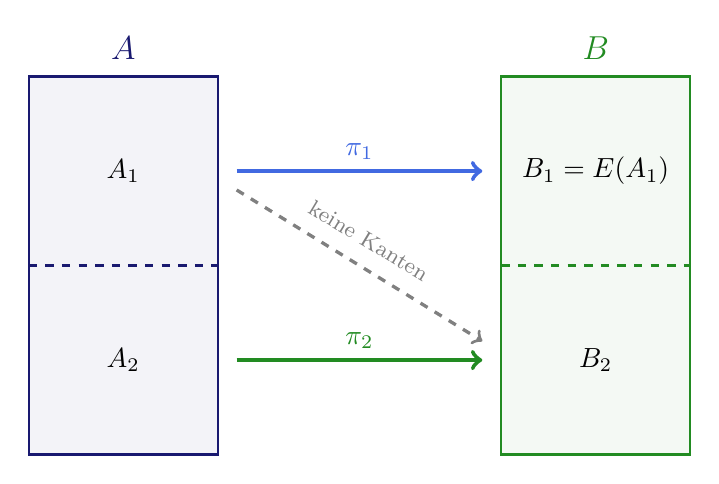
\begin{tikzpicture}[scale=1.2, thick]
  % [AI-TIKZ-PLANNER: Proof Case 2 (Partitioning of A and B)]
  % 1. Background: Split rectangles for A and B.
  % 2. Midground: Partition lines separating A1/A2 and B1/B2.
  % 3. Foreground: Mapping arrows showing the induction steps.
  
  % Set A
  \draw[thick, MidnightBlue, fill=MidnightBlue!5] (0,0) rectangle (2,4);
  \draw[dashed, MidnightBlue, thick] (0,2) -- (2,2);
  \node at (1,3) {\textbf{$A_1$}};
  \node at (1,1) {\textbf{$A_2$}};
  \node[MidnightBlue] at (1, 4.3) {\large $A$};

  % Set B
  \draw[thick, ForestGreen, fill=ForestGreen!5] (5,0) rectangle (7,4);
  \draw[dashed, ForestGreen, thick] (5,2) -- (7,2);
  \node at (6,3) {\textbf{$B_1 = E(A_1)$}};
  \node at (6,1) {\textbf{$B_2$}};
  \node[ForestGreen] at (6, 4.3) {\large $B$};

  % Mapping arrows
  \draw[->, ultra thick, RoyalBlue] (2.2,3) -- (4.8,3) node[midway, above] {$\pi_1$};
  \draw[->, ultra thick, ForestGreen] (2.2,1) -- (4.8,1) node[midway, above] {$\pi_2$};
  \draw[->, dashed, gray, line width=1.2pt] (2.2,2.8) -- (4.8,1.2);
  \node[gray, rotate=-31, above] at (3.5,2.1) {\footnotesize keine Kanten};
\end{tikzpicture}
\end{center}
\end{math-stroke}

\begin{spoken-clean}[01:15:02 - 01:17:32]
Nun wollen wir auf diese Teilmengen die Induktionsvoraussetzung anwenden. Wir wissen, dass $A_1$ eine echte Teilmenge von $A$ ist. Da $|A_1| < |A| = n+1$ gilt, hat $A_1$ höchstens $n$ Elemente. Da die Hall-Bedingung für den Gesamtgraphen $G$ gilt, gilt sie insbesondere auch für jede Teilmenge von $A_1$. Nach Induktionsvoraussetzung existiert daher eine Injektion $\pi_1 \colon A_1 \to B_1$ mit $\{a, \pi_1(a)\} \in E_1$ für alle $a \in A_1$.

Jetzt müssen wir noch zeigen, dass der verbleibende Teilgraph $G_2 = (A_2, B_2, E_2)$ ebenfalls die Hall-Bedingung erfüllt. Angenommen, dies sei nicht der Fall. Dann existiert eine Teilmenge $X \subseteq A_2$, für die gilt:
\[
|X| > |E_2(X)|.
\]
\end{spoken-clean}

\begin{spoken-clean}[01:17:32 - 01:20:02]
Wir betrachten nun die disjunkte Vereinigung $A_1 \cup X \subseteq A$. Da $A_1$ und $X$ disjunkt sind, gilt für die Kardinalität:
\[
|A_1 \cup X| = |A_1| + |X|.
\]
Nach unserer Annahme für Fall 2 gilt $|A_1| = |E(A_1)|$, und nach der Widerspruchsannahme gilt $|X| > |E_2(X)|$. Setzen wir das ein, erhalten wir:
\[
|A_1| + |X| > |E(A_1)| + |E_2(X)|.
\]
Da $E(A_1) \subseteq B_1$ und $E_2(X) \subseteq B_2$ disjunkt sind, ist die Summe ihrer Kardinalitäten genau gleich der Kardinalität ihrer Vereinigung:
\[
|E(A_1)| + |E_2(X)| = |E(A_1) \cup E_2(X)|.
\]
Da alle Kanten, die von $A_1 \cup X$ ausgehen, entweder in $B_1$ (was genau $E(A_1)$ entspricht) oder in $B_2$ (was $E_2(X)$ entspricht) landen müssen, ist $E(A_1 \cup X) \supseteq E(A_1) \cup E_2(X)$. Daraus folgt:
\[
|E(A_1) \cup E_2(X)| \le |E(A_1 \cup X)|.
\]
\end{spoken-clean}

\begin{spoken-clean}[01:20:02 - 01:22:32]
Zusammengenommen erhalten wir also:
\[
|A_1 \cup X| > |E(A_1 \cup X)|.
\]
Dies steht jedoch im direkten Widerspruch zur Hall-Bedingung für den Gesamtgraphen $G$, von der wir wissen, dass sie für alle Teilmengen erfüllt sein muss.

Unsere Widerspruchsannahme war also falsch, und der Teilgraph $G_2 = (A_2, B_2, E_2)$ erfüllt die Hall-Bedingung ebenfalls. Da $|A_2| \le n$ ist, existiert nach Induktionsvoraussetzung eine Injektion $\pi_2 \colon A_2 \to B_2$ mit $\{a, \pi_2(a)\} \in E_2$ für alle $a \in A_2$.

Nun können wir diese beiden Abbildungen zusammensetzen: Wir definieren die Abbildung $\pi \colon A \to B$ durch $\pi(a) := \pi_1(a)$, falls $a \in A_1$ ist, und $\pi(a) := \pi_2(a)$ andernfalls. Da $B_1$ und $B_2$ disjunkt sind, ist diese zusammengesetzte Abbildung ebenfalls injektiv und erfüllt $\{a, \pi(a)\} \in E$ für alle $a \in A$. Dies beendet den Beweis.
\end{spoken-clean}

\begin{math-stroke}[Induktionsschritt: Fall 2 Widerspruchsbeweis]
\begin{short-proof}[Beweis von Fall 2]
\textbf{Fall 2: Existenz einer scharfen Schranke für eine echte Teilmenge.}
Es existiere eine echte Teilmenge $\emptyset \neq A_1 \subsetneq A$ mit $|A_1| = |E(A_1)|$.
\par\vspace{1ex}\noindent
Wir definieren die disjunkten Partitionen:
\begin{align*}
B_1 &:= E(A_1) \\
A_2 &:= A \setminus A_1 \\
B_2 &:= B \setminus B_1
\end{align*}
Sowie die induzierten Kantenmengen $E_1 := E \cap (A_1 \times B_1)$ und $E_2 := E \cap (A_2 \times B_2)$.
\par\vspace{1ex}\noindent
Da $|A_1| < |A|$, existiert nach Induktionsvoraussetzung eine Injektion $\pi_1 \colon A_1 \to B_1$ mit $\{a, \pi_1(a)\} \in E_1$ für alle $a \in A_1$.
\par\vspace{1ex}\noindent
Wir zeigen nun, dass der Teilgraph $G_2 = (A_2, B_2, E_2)$ ebenfalls die Hall-Bedingung erfüllt. Angenommen, dies sei nicht der Fall. Dann existiert eine Teilmenge $X \subseteq A_2$ mit:
\begin{equation}\label{eq:contradiction-assumption}
|X| > |E_2(X)|.
\end{equation}
Wir betrachten die disjunkte Vereinigung $A_1 \cup X \subseteq A$. Es gilt:
\begin{align}
|A_1 \cup X| &= |A_1| + |X| \nonumber \\
&> |E(A_1)| + |E_2(X)| \quad \text{(wegen \eqref{eq:contradiction-assumption} und } |A_1| = |E(A_1)|) \nonumber \\
&= |E(A_1) \cup E_2(X)|. \label{eq:union-ineq}
\end{align}
Da alle Kanten von $A_1 \cup X$ entweder in $B_1 = E(A_1)$ oder in $B_2$ landen müssen, gilt $E(A_1 \cup X) \supseteq E(A_1) \cup E_2(X)$. Daraus folgt mit \eqref{eq:union-ineq}:
\[
|A_1 \cup X| > |E(A_1 \cup X)|.
\]
Dies steht im Widerspruch zur Hall-Bedingung für den Gesamtgraphen $G$. Somit erfüllt $G_2$ die Hall-Bedingung, und nach Induktionsvoraussetzung existiert eine Injektion $\pi_2 \colon A_2 \to B_2$ mit $\{a, \pi_2(a)\} \in E_2$ für alle $a \in A_2$.
\par\vspace{1ex}\noindent
Die zusammengesetzte Abbildung $\pi \colon A \to B$ mit:
\[
\pi(a) := \begin{cases}
\pi_1(a) & \text{falls } a \in A_1 \\
\pi_2(a) & \text{falls } a \in A_2
\end{cases}
\]
ist injektiv und erfüllt $\{a, \pi(a)\} \in E$ für alle $a \in A$.
\end{short-proof}
\end{math-stroke}
\end{proof}

\begin{spoken-clean}[01:24:49 - 01:26:33]
Ja, schauen Sie sich den Beweis nochmals in Ruhe an --- er ist nicht so schwierig, aber wirklich elegant, wie das alles aufgeht. Ein sehr schöner Induktionsbeweis mit diesen beiden Fallunterscheidungen.

Sie sind diesem Satz vielleicht auch schon einmal begegnet. Es ist ein sehr berühmtes Resultat, für das es viele verschiedene Beweise gibt --- wenn Sie im Internet nach \qt{Beweise des Heiratssatzes} suchen, finden Sie bestimmt sehr schnell zehn verschiedene Ansätze und Varianten.

Gut, so weit zur Graphentheorie. Machen Sie bitte die Übungsaufgaben; es sind ein paar nette Aufgaben zur Graphentheorie dabei, um einfach mit dieser Art von Mathematik etwas vertrauter zu werden. Nächste Woche machen wir dann mit elementarer Zahlentheorie weiter.

Vielen Dank und eine schöne Woche!
\inlinemetanote{Die Studenten applaudieren, der Dozent packt seine Unterlagen ein}
\end{spoken-clean}

\begin{didactic-insight}[Die mathematische Tiefe des Heiratssatzes]
Der Heiratssatz von Hall (1935) ist ein zentrales Resultat der diskreten Mathematik und der Kombinatorik. Er ist äquivalent zu vielen anderen fundamentalen Sätzen, wie dem \newterm{Max-Flow-Min-Cut-Theorem} von Ford und Fulkerson, dem \newterm{Satz von Menger} über disjunkte Pfade und dem \newterm{Satz von Dilworth} über Antiketten in Halbordnungen. Die hier gezeigte Induktionsmethode über die Kardinalität der Knotenmenge verdeutlicht die strukturelle Eleganz kombinatorischer Beweise.
\end{didactic-insight}

\begin{nice-box}[Zusammenfassung der Schlüsselkonzepte]
In dieser Vorlesung haben wir vier fundamentale Themenbereiche der Graphentheorie behandelt:
\begin{enumerate}[label=\textbf{(\arabic*)}]
    \item \textbf{Das Handschlaglemma:} In jedem endlichen Graphen ist die Anzahl der Knoten mit ungeradem Grad stets gerade. Dies folgt direkt aus der Tatsache, dass die Summe aller Knotengrade genau das Doppelte der Kantenanzahl beträgt.
    \item \textbf{Euler-Graphen:} Ein zusammenhängender Graph besitzt genau dann eine geschlossene Euler-Linie (einen Kantenzug, der jede Kante exakt einmal enthält), wenn jeder Knoten einen geraden Grad aufweist.
    \item \textbf{Hamilton-Graphen:} Ein Graph ist hamiltonsch, wenn er einen Kreis besitzt, der jeden Knoten exakt einmal besucht. Wir haben gezeigt, dass der $k$-dimensionale Hyperwürfel $Q_k$ stets hamiltonsch ist, was äquivalent zur Existenz eines zyklischen Gray-Codes ist.
    \item \textbf{Der Heiratssatz von Hall:} Ein bipartiter Graph $G = (A, B, E)$ besitzt genau dann ein perfektes Matching (eine Injektion von $A$ nach $B$ entlang der Kanten), wenn für jede Teilmenge $X \subseteq A$ die Hall-Bedingung $|X| \le |E(X)|$ erfüllt ist.
\end{enumerate}
\end{nice-box}

% [SYSTEM] Refinement complete